\documentclass[a4paper,12pt]{article}

\usepackage{tkz-euclide}
\usepackage{gensymb}
\usepackage[utf8]{inputenc}
\usepackage{graphicx}

\title{ASSIGNMENT-3}
\author{SENANI SADHU}
\date{\today}
\begin{document}
	\maketitle
	\pagenumbering{roman}
	\section{Question:-}
	\paragraph{In $\Delta$ABC, given that a+b+c = 11, $\angle$B = 45$^{\circ}$ 
		and
		$\angle$C = 45$^{\circ}$ 
		, find a, b, c and sketch the triangle.}
	\section{Solution:-}
	\begin{tikzpicture}[scale=2]
		
		%Triangle sides
		\def\b{4}
		\def\c{3}
		
		%Marking coordiantes
		\coordinate [label=above:$B$] (B) at (0,\c);
		\coordinate [label=left:$A$] (A) at (0,0);
		\coordinate [label=right:$C$] (C) at (\b,0);
		
		%Drawing triangle ABC
		\draw (B) -- node[left] {$\textrm{c}$} (A) -- node[below] {$\textrm{b}$} (C) -- node[above,,xshift=2mm] {$\textrm{a}$} (B);
		
		%Drawing and marking angles
		\tkzMarkAngle[fill=orange!40,size=0.5cm,mark=](B,C,A)
		\tkzMarkRightAngle[fill=blue!20,size=.3](B,A,C)
		\tkzLabelAngle[pos=0.65](B,C,A){ 45$^{\circ}$ }
		\tkzMarkAngle[fill=orange!40,size=0.5cm,mark=](A,B,C)
		\tkzLabelAngle[pos=0.65](A,B,C){ 45$^{\circ}$ }
	\end{tikzpicture}
\newline
Given, 
\begin{equation}
	a+b+c=11
\end{equation}
\newline
We know that, 
\newline
tan(ACB)=$\frac{c}{b}$
\newline
tan(45$^{\circ}$)=$\frac{c}{b}$
\begin{equation}
	c=b
\end{equation}
\newline
Now, $a^2$=$c^2$+$b^2$   (Pythagoras Theorem)
\newline
Using eq 2) 
\begin{equation}
	$$2$b^2$=$a^2$$$
\end{equation}
Also, eq 1) becomes 
\begin{equation}
	a=11-2b    
\end{equation}
\newline
Therefore, eq 3) becomes
\newline
2$b^2$=$(11-2b)^2$
\newline
2$b^2$-44b+121=0
\newline
b=3.22,b$\neq$18.78
\newline
a=11-2*3.22=4.56
\newline
\paragraph{a=4.56 , c=3.22 , b=3.22}
\subsection{Steps of Construction:-}
\begin{itemize}
	\item Draw a line BC of length b=4.5.
	\item Taking B as centre draw an arc at the distance of as c=3.25.
	\item Taking C as centre draw an arc at the distance of as a=3.25.
	\item Name the point where the two arcs meet as A.
	\item Join AB and AC.
	\item Join AB and AC.
\end{itemize}
\subsection{Figure:-}
\begin{center}
	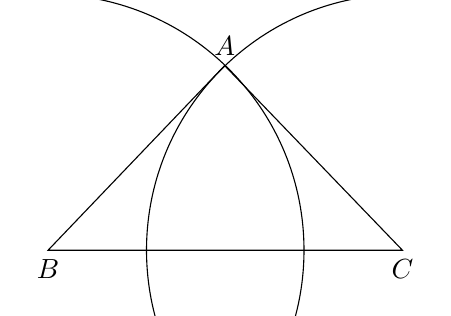
\begin{tikzpicture}[scale=1]
		\coordinate[label=below:$B$] (b) at (0,0);
		\coordinate[label=below:$C$] (c) at (4.5,0);
		\begin{pgfinterruptboundingbox}
			\node(Cric1) at (b) [draw, circle through=($ (b) + (0:3.25) $)] {};
			\node(Cric2) at (c) [draw, circle through=($ (c) + (0:3.25) $)] {};
		\end{pgfinterruptboundingbox}
		\coordinate[label=above:$A$] (a) at (intersection 2 of Cric1 and Cric2);
		\draw(b)--(a)--(c)--cycle;
	\end{tikzpicture}
\end{center}

\end{document}